% Выбор класса документа
%\documentclass {book}
%\documentclass {article}
\documentclass [a4paper, 12pt, oneside]{scrbook}
% Чтобы можно было использовать русские буквы в формулах,
%но в случае использования предупреждать об этом
\usepackage [warn]{mathtext}
% Выбор внутренней TEX−кодировки
\usepackage[T2A]{fontenc}
% Выбор кодовой страницы документа
% Так же можно выбрать cp1251 или utf8
\usepackage[utf8]{inputenc}
% Выбор языка документа
\usepackage[english,russian]{babel}
% Начинать первый параграф
\usepackage{indentfirst}

% Загрузка пакета hyperref
\usepackage[unicode=true] {hyperref}
%\usepackage{url}
\usepackage{colortbl}
\usepackage{tabularx}

\usepackage{graphicx}
\graphicspath{pictures/}
\DeclareGraphicsExtensions{.pdf,.png,.jpg}

%\makeatletter
%\renewcommand*{\@biblabel}[1]{\hfill#1.}
%\makeatother

%\usepackage[backend=biber]{biblatex}
%\addbibresource{references.bib}

%установка тире для подрисуночной подписи
\RequirePackage{caption}
\DeclareCaptionLabelSeparator{defffis}{ --- }
\captionsetup{justification=centering,labelsep=defffis}

\usepackage{csquotes}
\usepackage{debate}
\usepackage[nopygments,nonumbers,noframes]{ffcode}
\usepackage{to-be-determined}
\usepackage{inputenc}

\usepackage{longtable}
\usepackage{hhline}

\newcommand\code[1]{\ff{#1}}

% Конец преамбулы и начало документа
\begin {document}

% Изменение начала подрисуночной надписи
\renewcommand\figurename{Рисунок}

% --- Титульная страница -----------------------------------

\title{\Huge{Архитектура вычислительных систем\\ \large{Методические указания к самостоятельной работе студентов}}}

\author {{\Large{А.\,И.~Легалов}}
    \and {\Large{С.\,А.~Виденин}}
    \and {\Large{К.\,И.~Пашигорев}}}

%\date {13.08.2022}
\maketitle

% --- Оглавление -------------------------------------------

\tableofcontents

% Основная часть
%\mainmatter

% --- Введение -------------------------------------------
% Введение

\chapter* {Введение}
\addcontentsline{toc}{chapter}{Введение}

Вычислительные системы (ВС) различного назначения в настоящее время используются практически повсеместно. Они сопровождают нас в повседневной жизни, используются в промышленности и в быту, поддерживают игровой контент и решение экономических проблем. Несмотря на их разнообразие существуют некоторые общие принципы, связанные с особенностями организации и построения вычислительных систем, которые необходимо знать для повышения эффективности их использования. Эти принципы отражаются в архитектурных решениях, обеспечивающих представление как внутренней структуры ВС так и их взаимодействия с пользователями, которыми в большинстве своем являются программистами.

\section*{Цель и задачи}

Целью дисциплины является изучение особенностей архитектур вычислительных систем, их многоуровневости и разнообразия. Для достижения поставленной цели предполагается рассмотреть следующие основные разделы:

\begin{itemize}
 \item Общее понятие архитектуры ВС. Классификация архитектур ВС
 \item Особенности архитектуры ВС уровня системы команд.
 \item Отображение архитектуры ВС уровня системы команд в языках системного программирования и ассемблере.
 \item Уровень операционной системы и его использование в низкоуровневом программировании.
 \item Разнообразие архитектур уровня системы команд.
 \item Поддержка архитектуры уровня системы команд на уровне микроархитектур.
 \item Отображение параллелизма в архитектурах ВС.
\end{itemize}


\section*{Основные темы, затрагиваемые при изучении дисциплины}

При всей многоуровневости и разнообразии архитектур ВС рамках изучаемой дисциплины основной упор предполагается сделать на уровень системы команд и параллелизм. Это обуславливается тем, что в объеме одного семестра можно либо глубоко рассмотреть ограниченный набор архитектурных решений, либо поверхностно пробежаться по более широкому их числу, избегая конкретики. Я предпочитаю первый вариант. Исходя из этого самым верхним будет являться архитектурный уровень языков системного программирования, который рассматривается как основополагающая связь между более верхними уровнями прикладных языков и всем тем, что находится ниже.

В качестве языка программирования, отражающего системный уровень выбран язык C, который практически однозначно отображает в своих конструкциях низкоуровневые решения. Он позволяет рассмотреть использование библиотек, определяющих архитектуры уровня операционной системы (ОС), а также продемонстрировать непосредственную связь с языками ассемблера для различных архитектур уровня системы команд. Помимо этого использование данного языка позволяет применить его библиотеку функций при программировании на языке ассемблера, обеспечивая более высокоуровневый ввод-вывод данных, работу с файлами, а также ряд других манипуляций по сравнению с использованием аналогичных системных вызовов уровня операционной системы.

Рассмотрение уровня операционной системы позволяет рассмотреть реализацию параллелизма, что в настоящее время является неотъемлимой практикой в программировании. Помимо системных вызовов предполагается также рассмотреть более высокоуровневую поддержку параллельных вычислений для различных архитектур, которая опирается на системные вызовы ОС.


Практические занятия и задания

В рамках практических занятий основной упор делается на выполнение заданий, закрепляющих знания низкоуровневых архитектур, таких как уровень ОС, ассемблера, системы команд. Для написания программы при этом используется язык ассемблера. Помимо этого имеются задания связанные с изучением и практическим использованием многопоточных архитектур на уровне ОС и библиотеки Posix threads. Используемое при этом многопоточное программирования осуществляется на языке программирования C.

При выполнении заданий предполагается использование следующих инструментальных средств и систем программирования:

\begin{itemize}
 \item вычислительную систему (ПК, ноутбук) с архитектурой x86-64 (AMD-64);
\item операционную систему Linux;
\item языки программирования C (gcc, clang), GNU ассемблер (as);
\item библиотеки уровня ОС и языка C (stdio.h, stdlib.h, string.h и т.д.)
\end{itemize}

Выбор архитектуры машинного уровня x86-64 обуславливается ее массовым распространением, что позволяет не использовать различные эмуляторы и упрощает непосредственное взаимодейстивие с компьютером.

Свободно распространяемой ОС Linux вполне достаточно для решения заданий. Помимо возможной непосредственной установки ее можно легко запускать в различных эмулирующих средах. В частности, под ОС Windows можно использовать Windows Subsystem for Linux (WSL). На любой платформе можно также запускать Linux под виртуальной машиной, например, VirtualBox. Описания вариантов установки доступны в сети Интернет. Практически можно использовать любой дистрибутив. При этом достаточно консольной версии, так как в результате выполнения заданий должны создаваться только консольные приложения.

Компиляторы языков программирования C имеются практически в любом дистрибутиве Linux. Проще при этом ориентироваться на семейство Gnu Compiler Collection (GCC). Однако можно использовать и clang.

Среди всего разнообразия ассемблеров, которые используются в ОС Linux, предлагается ориентироваться на тот из них, который по сути является основным инструментом в данной операционной системе. Это GNU ассемблер (GAS). В этом случае программы, разрабатываемые непосредственно на ассембле, можно легко сопоставлять с программами, написанными на C и откомпилированными в ассемблер, что позволяет быстрее изучать и отыскивать необходимые машинные команды по аналогии. Также следует отметить, что язык C позволяет использовать ассемблерные вставки, написанные на GAS, что также облегчает изучение архитектур уровней ассемблера и системы команд. Помимо этого основной отладчик в Linux, Gnu Debugger (gdb), так же поддерживает мнемонику данного ассемблера. При этом выбор мнемоники (intel или AT\&T(?)). Можно осуществлять по собственному усмотрению.

Состав библиотек определяется тем, что они поддерживаются практически всеми компиляторами C, обеспечивая также работу с языками ассемблера.

Предлагаемые задания достаточно простые и не требуют для их написания интегрированных средств разработки. Достаточно текстовых редакторов. В качестве дополнительных инструментов могут опционально пригодиться средства сборки проектов cmake и make. Для сохранения результатов работы и обеспечения их проверки необходимо пользоваться одной из систем контроля версий в сети Интернет (предлагается использовать github).

\section*{Краткое содержание курса}

\begin{center}
\fbox{%
    \parbox{15cm}{\textit{\textbf{Примечание}}

        Пока оставил текст из предыдущего описания. Нужно продумать и разделить, что пойдет в ЛМС, а что на сайт. Предполагается, что на сайте будет выложен более подробный материал. Болшее число тем.}
}
\end{center}

Основной упор я предполагаю сделать на традиционных архитектурах в разрезе их многоуровневости. То есть, пройтись по вертикали от логических схем и архитектуре на уровне этих схем, рассмотрев построение систем на кристалле. На верхнем уровне, скорее всего, будут специализированные архитектуры и архитектуры параллельных вычислительных систем. С каждым из уровней предполагается увязать свой язык программирования, рассмотреть основной набор команд и обобщенную структуру виртуальной машины данного уровня.

Изложение скорее всего не будет упорядочено по уровням (сверху вниз или снизу вверх). Я планирую отталкиваться от известных архитектур универсальных языков высокого уровня, опускаясь в начале до командного уровня (до языков ассемблера). На уровне системы команд предполагаю разобрать различные варианты современных архитектур.

Исходя из этого планируется следующая последовательность подачи материала в лекционном курсе.

\subsubsection*{Архитектура процедурной императивной машины}

В рамках данной темы планируется затронуть упрощенную организацию высокоуровневой императивной машины, использующей статическую типизацию данных. Начать стоит с «Фортран-машины», то есть, с нулевого метауровня, не содержащего абстракция более высоко уровня. Показать отличия систем типов на основе методов задания однозначности. Рассмотреть особенности структур различного вида: бестиповой, статически типизированной, динамически типизированной. Увязать их с различными видами архитектур. Рассмотреть соответствующие примеры на языках C++ (в стиле C), Python (или JS). пояснить, почему динамическая типизация чаще используется в интерпретируемых языках.

Может быть при анализе типов также стоит отметить, что между статической и функциональной однозначностью существуе однозначный переход.

После этого можно перейти к первому метауровню, на котором рассматриваются абстрактные типы данных. В этот же метауровень можно внести формальные параметры функций (процедур). Рассмотреть структурную организацию и обобщенную архитектурную поддержку. Показать, как данный метауровень реализуется в статически типизированных процедурныъ языках на агрегативных данных (структурах), пояснив его суть. Пояснить, почему он не используется особо в языках с динамической типизацией.

После этого можно перейти к использованию АТД для описания альтернативных типов данных. Пояснить, что в любой мало-мальски приличной программе всегда необходима проверка типов во время выполняения. Продемонстрировать на примере. Пояснить растипизацию (разыменование типов). Показать наличие растипизации и необходимость дополнительных механизмов проверки типов. Рассказать о бестиповом подходе с явным заданием признака. Также рассказать о более надежном решении, которое используетс в языке программирования Ада.

Помимо этого можно сопоставить императивный и функциональный подход. Показать, в чем заключается основная специфика функционального программирования и его отличия от процедурного. Разобрать архитектуры функциональных машин. Показать, что в них также может использоваться различная система типов.

В качестве задания и тем для обсуждения на практических занятиях планируется предложить разработку программы для процедурной машины. Может быть для разнообразия в качестве альтернативных решений стоит добавить использование различных систем типов и уровней абстракции (м.б. и языков программирования). Хотя, скорее всего основная идея - это использование статической типизации и абстрактных типов данных при процедурном подходе.


\subsubsection*{Архитектура объектно-ориентированной машины}

\subsubsection*{Архитектура уровня системы команд}

\subsubsection*{Архитектура уровня микрокоманд}

\subsubsection*{Архитектура логического уровня}

\subsubsection*{Архитектуры параллельных вычислительных систем}

\section*{Зачем читать эту книгу?}

Учитывая, что существует множество отличных языков высокого уровня, которые позволяют вам писать программы, не заботясь о том, как машинные инструкции управляют оборудованием, вы можете задаться вопросом, зачем вам изучать материал этой книги. Все языки высокого уровня в конечном счете переводятся в машинные инструкции, управляющие оборудованием. \textbf{\textit{Понимание того, что делает аппаратное обеспечение и как инструкции управляют им, поможет понять возможности и ограничения компьютера. Я считаю, что это понимание может сделать вас лучшим программистом, даже если вы работаете с языком высокого уровня.}}

Если вас в первую очередь интересует аппаратное обеспечение, я думаю, важно понимать, как аппаратное обеспечение будет использоваться программой.

Вам может понравиться программирование на ассемблере, и вы захотите продолжить. Например, если ваши интересы приводят вас к системному программированию — написанию частей операционной системы, написанию компилятора или даже разработке другого языка более высокого уровня — эти усилия обычно требуют понимания на уровне языка ассемблера.

Много сложных возможностей также существует в программировании встроенных систем, систем, в которых компьютер выполняет специальную задачу. Примеры являются неотъемлемой частью нашей повседневной жизни: сотовые телефоны; бытовая техника; автомобили; системы отопления, вентиляции и кондиционирования воздуха (HVAC); медицинское оборудование; и так далее. Встроенные системы являются важным компонентом технологии Интернета вещей (IoT). Их программирование часто требует понимания того, как компьютер взаимодействует с различными аппаратными устройствами на уровне языка ассемблера.

% --- Представление данных в вычислительных системах ---
%\chapter{Представление данных в вычислительных системах}



\section{Представление целочисленных данных}

В этом разделе описываются два разных способа использования битов для представления целых чисел: один из этих способов позволяет представлять только неотрицательные числа, а другой --- отрицательные числа, положительные и ноль. Позже мы увидим, что они сильно взаимосвязаны как математическими свойствами, так и реализациями на машинном уровне. Мы также рассмотрим влияние расширения или сжатия целых чисел, чтобы их можно было уместить в представления с разной длиной.

\subsection{Представление целых без знака}

Пусть имеется целочисленный тип, представляющий значения из w бит. Битовый вектор записывается либо как $\vec{x}$, что обозначает вектор как единое целое, либо как $[x_{n-1}, x_{n-2}...x_0]$ с перечислением отдельных битов в векторе. Рассмотрим $\vec{x}$ как число, записанное в двоичном виде. В этом случае мы получим интерпретацию $\vec{x}$ как числа без знака. Каждый бит $x_i$ имеет значение 0 или 1. В последнем случае он соответствует величине $2^i$, которая является составной частью всего числа.



\section{Представление значений с плавающей точкой. Cтандарт IEEE}

Позиционное представление, подобное рассмотренному в предыдущем разделе, неэффективно для очень больших чисел. Например, представление $5 × 2^{100}$ будет состоять из комбинации битов 101, за которой следует 100 нулей. Вместо этого предпочтительнее представлять такие числа в форме $x × 2^y$ путем задания значений х и y.

Стандарт IEEE определяет представление чисел с плавающей точкой в виде:
\begin{center}
    \large{$V = (-1)^s × M × 2^E$}
\end{center}
где:
\begin{itemize}
    \item символ $s$ определяет знак числа, который может быть отрицательным при $s = 1$ или положительным при $s = 0$ (интерпретация знакового разряда для числового значения 0 рассматривается как особый случай);
    \item мантисса М --- дробное двоичное число в диапазоне от 1 до 2 – $\varepsilon$ или от 0  до 1 – $\varepsilon$ (значение $\varepsilon$ определяет точность вычислений и зависит от разрядности мантиссы);
    \item показатель Е – взвешивает величину (возможно, отрицательной)  степенью 2.
\end{itemize}

Для кодировки этих величин битовое представление числа с плавающей точкой делится на три поля:

\begin{itemize}
    \item знаковый бит s напрямую кодирует символ s;
    \item k-разрядное поле показателя $ехр = e_{k-1} ... e_1e_0$ кодирует показатель Е;
    \item n-разрядное поле дробной части $frac = f_{n-1} ... f_1f_0$ кодирует мантиссу М, способ кодирования также зависит от того, равно поле показателя 0 или нет.
\end{itemize}

На рис~\ref{data01}. 2.13 показано, как эти три поля упакованы в два наиболее распространенных формата. В формате с одинарной точностью (тип float в языке С) поля s, exp и frac имеют размеры 1, k = 8 и n = 23 бит, что дает 32-разрядное представление. В формате с двойной точностью (тип double в языке С) поля s, ехр и frac имеют размеры 1, k = 11, n = 52 бит, что дает 64-разрядное представление.

\begin{figure}[htbp]
    \centering
    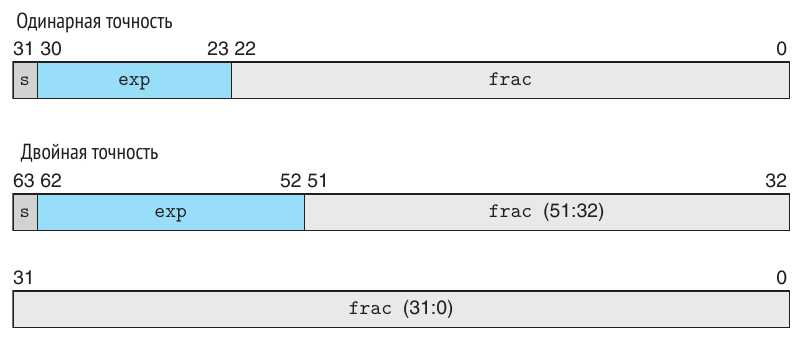
\includegraphics[width=0.8\textwidth]{img/data01.png}
    \caption{Стандартные форматы представления чисел с плавающей запятой}
    \label{data01}
\end{figure}

Величину, представленную конкретным битовым представлением, можно разделить на три разных варианта (последний имеет два подварианта), в зависимости от значения ехр. Они показаны на рисунке~\ref{data02}.

\begin{figure}[htbp]
    \centering
    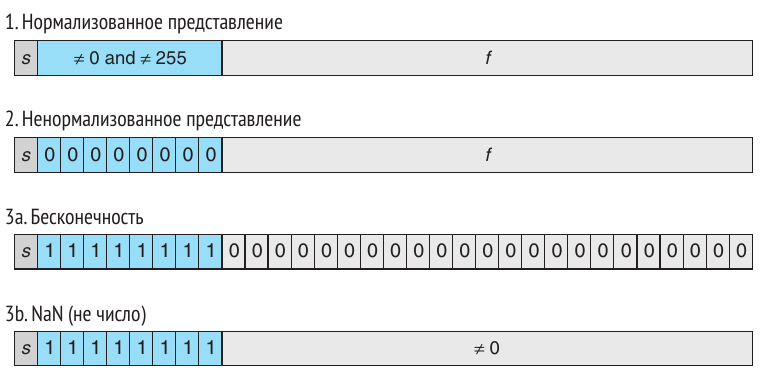
\includegraphics[width=0.8\textwidth]{img/data02.png}
    \caption{Категории значений с плавающей запятой одинарной точности. Значение показателя определяет, является число (1) нормализованным, (2) ненормализованным или (3) особым}
    \label{data02}
\end{figure}

\subsection{Вариант 1: нормализованные значения}

Это самый общий случай. Он имеет место, когда комбинация битов ехр состоит либо из одних нулей (числовое значение 0), либо из одних единиц (числовое значение 255 для одинарной точности и 2047 для двойной). В этом случае поле показателя интерпретируется как целое со знаком в смещенной форме. То есть показатель имеет значение $Е = е - Bias$ (смещение), где $е$ – число без знака с битовым представлением $e_{k-1} ... e_1e_0$, a $Bias$ --- величина смещения, равная $2^{k-1} - 1$ (127 для одинарной точности, 1023 --- для двойной). Это разложение дает диапазон показателей от -126 до +127 для одинарной точности и от -1022 до +1023 – для двойной.

Поле дробной части frac интерпретируется как представляющее дробную величину f, где $0 \leq f < 1$, имеющую двоичное представление $0.f_{n-1} ... f_1f_0$, т.~ е. с двоичной точкой слева от самого значимого бита. Мантисса определяется как $М = 1 + f$. Иногда такое представление называют представлением с неявной ведущей единицей, потому что M можно рассматривать как число с двоичным представлением $1.f_{n-1}f{n-2} ... f_0$. Такое представление позволяет получить дополнительный бит точности, поскольку показатель Е всегда можно настроить так, чтобы мантисса М находилась в диапазоне $1 \leq M < 2$ (при условии отсутствия переполнения). Поэтому нет необходимости явно представлять ведущий, так как он всегда равен единице.

\begin{center}
\framebox[\textwidth][l]{
\begin{minipage}{0.95\linewidth}
\textbf{Зачем устанавливать смещение для ненормализованных значений}

Использование значения показателя 1 - Bias вместо простого -Bias может показаться противоречащим здравому смыслу. Но очень скоро вы увидите, что такое представление упрощает переход от ненормализованных значений к нормализованным.
\end{minipage}
}
\end{center}

\subsection{Вариант 2: ненормализованные значения}

Когда поле показателя состоит только из нулей, то представляемое число находится
в ненормализованной форме. В этом случае значение порядка Е = 1 - Bias, а значение мантиссы M = f, т. е. значение дробной части не имеет неявной ведущей единицы.

Ненормализованные значения служат двум целям. Во-первых, они позволяют представлять числовое значение 0, поскольку для нормализованного представления всегда выполняется условие $M \geq 1$, и, следовательно, оно не позволяет представить 0. Фактически представление чисел с плавающей точкой +0.0 имеет комбинацию битов, состоящую из одних нулей: знаковый разряд содержит 0, поле показателя
полностью состоит из нулей (что указывает на ненормализованное значение), и поле дробной части тоже состоит из одних нулей, давая M = f = 0. Интересно, что когда знаковый разряд равен единице, а все другие поля – нулю, то получается значение -0.0. В формате IEEE с плавающей точкой значения -0.0 и +0.0 в одних случаях
рассматриваются как разные, а в других – как одинаковые.

Вторая цель, которую преследуют ненормализованные значения, – представление чисел, близких к 0.0. Они обеспечивают свойство равномерного приближения к нулю, при котором возможные числовые значения равномерно располагаются около 0.0.

\subsection{Вариант 3: особые значения}

Последняя форма представления значений используется, когда поле показателя со
стоит из одних единиц. Если при этом поле дробной части состоит из одних нулей, то в результате получается бесконечность: либо $+\infty$, когда s = 0, либо $-\infty$, когда s = 1. Бесконечность может представлять переполнение как при умножении очень больших чисел, так и при делении на ноль. Когда дробная часть не равна нулю, то такое значение называется NaN (сокращенно <<Not a Number>> – не число). Такие значения возвращаются, когда результат операции нельзя представить вещественным числом или бесконечностью, как, например, $\sqrt{-1}$ или $\infty - \infty$. Они также могут пригодиться в некоторых приложениях для инициализации данных.

% --- Эмулятор RARS процессора RISC-V ---
\chapter{Эмулятор RARS процессора RISC-V}

RARS --- это интегрированная среда разработки, отладки и выполнения программ процессора RISC-V в режиме симуляции. Она написана на языке программирования Java, что обеспечивает переносимость между компьютерами с различной архитектурой, использующих разнообразные операционные системы. Распространяется в виде исполняемого файла JAR. Среда включает:
\begin{itemize}
    \item текстовый редактор, обеспечивающий написание программ;
    \item ассемблер, позволяющий получить исполняемый код путем сборки одного или нескольких модулей;
    \item эмулятор, осуществляющий моделирование процессора RISC-V и позволяющий выполнять программы, разработанные на языке ассемблера;
    \item отладчик, работающий как в пошаговом режиме, так и использующий точки останова;
    \item средства, обеспечивающие отображение информации о состоянии регистров моделируемого процессора и его оперативной памяти;
    \item модели внешних устройств, позволяющие имитировать взаимодействие с внешней средой в различных режимах.
\end{itemize}
Помимо этого компоненты, входящие в среду разработки можно запускать из командной строки.
\debate[Примечание]{Остальне будет дописываться по мере развития методы...}

\section{Использование RARS через интегрированную среду разработки (IDE)}

IDE вызывается, когда RARS запускается без аргументов команды, например: \verb|java -jar rars.jar|. Его также можно запустить из графического интерфейса, дважды щелкнув значок \verb|rars.jar|, представляющий этот исполняемый файл JAR. IDE предоставляет интуитивно понятные базовые возможности редактирования, сборки и выполнения. Ниже представлены некоторые доступные функции:
\begin{itemize}
    \item \textbf{Меню и панель инструментов.} Большинство элементов меню имеют одинаковые значки на панели инструментов. Если функция значка на панели инструментов не очевидна, просто наведите на него указатель мыши, и вскоре появится всплывающая подсказка. Почти все пункты меню также имеют сочетания клавиш. Любой пункт меню, не подходящий в данной ситуации, отключается.
    \item \textbf{Редактор.} RARS включает два встроенных текстовых редактора. Редактор по умолчанию имеет цветовую подсветку большинства языковых элементов с учетом синтаксиса и всплывающие инструкции. Помимо этого имеется ранее разработанный универсальный текстовый редактор без этих функций. Его можно выбрать в диалоговом окне <<Настройки редактора>>. Он поддерживает один шрифт, который можно изменить в диалоговом окне настроек редактора. Нижняя граница каждого из этих редакторов включает строку курсора и положение столбца. Также отображаются номера строк. \textit{Можно использовать внешний редактор. RARS предоставляет удобную настройку, которая будет автоматически собирать файл, как только он будет открыт. См. меню <<Настройки>>.}
    \item \textbf{Области сообщений.} В нижней части экрана есть две области сообщений с вкладками. Вкладка <<\textbf{Run~I/O}>> используется во время выполнения для отображения ввода--вывода консоли по мере выполнения программы. Также имеется возможность осуществлять консольный ввод во всплывающем диалоговом окне, а затем отображать его в области сообщений. Вкладка с названием <<\textbf{Сообщения~RARS}>> используется для других сообщений, таких как ошибки сборки или выполнения, а также для информационных сообщений. Вы можете нажать на сообщения об ошибках сборки, чтобы выбрать соответствующую строку кода в редакторе.

    \item \textbf{Регистры.} Регистры отображаются постоянно, даже тогда, когда программа редактируется, а не запускается. При написании программы это служит полезным справочником по именам регистров и их обычному использованию (можно навести указатель мыши на имя регистра, чтобы увидеть всплывающие подсказки). Имеется три вкладки регистров:
    \begin{itemize}
        \item файл регистров, содержащий целочисленные регистры от \verb|x0| до \verb|x31|, регистры \verb|LO| и \verb|HI|, а также счетчик программ (\verb|pc|);
        \item \textit{выбранные регистры сопроцессора 0 (исключения и прерывания)};
        \item регистры с плавающей запятой сопроцессора 1.
    \end{itemize}
    \item \textbf{Сборка.} Выберите <<Собрать>> в меню <<Выполнить>> или соответствующий значок на панели инструментов, чтобы собрать файл, который в данный момент находится на вкладке <<Правка>>. Файлы в текущем каталоге. Если параметр <<Собрать все>> включен, ассемблер соберет текущий файл как <<основную>> программу, а также соберет все другие файлы сборки (\verb|*.asm|; \verb|*.s|) в том же каталоге. А с опцией <<Assemble Open>>, открытый в данный момент ассемблер также соберет открытые в данный момент файлы. Результаты связаны, и если все эти операции были успешными, программа может быть выполнена. На метки, объявленные глобальными с помощью директивы \verb|.globl|, можно ссылаться в любом другом файле проекта. Существует также параметр, разрешающий автоматическую загрузку и сборку выбранного файла обработчика исключений.
    \item \textbf{Выполнение.} После успешной сборки программы инициализируются регистры и заполняются три окна на вкладке <<Выполнение>>: текстовый сегмент, сегмент данных и метки программы. Основные функции времени выполнения описаны ниже.
    \item \textbf{Окно меток.} Отображение окна меток (таблица символов) управляется через меню настроек. При отображении вы можете щелкнуть любую метку или связанный с ней адрес, чтобы отцентрировать и выделить содержимое этого адреса в окне «Текстовый сегмент» или в окне «Сегмент данных» в зависимости от ситуации.
\end{itemize}
    Ассемблер и симулятор вызываются из IDE, когда вы выбираете операции Assemble, Go или Step в меню Run или соответствующие им значки на панели инструментов или сочетания клавиш. Сообщения RARS отображаются на вкладке Сообщения RARS области сообщений в нижней части экрана. Ввод и вывод консоли среды выполнения обрабатывается на вкладке Run I/O.

\section{Интерактивные функции отладки}

RARS предоставляет множество функций для интерактивной отладки на панели <<Выполнение>>:
\begin{itemize}
    \item В пошаговом режиме выделяется следующая команда для выполнения, а содержимое памяти обновляется на каждом шаге.
    \item Для непрерывного выполнения выбирает опция <<Go>>. Еe также можно использовать для продолжения выполения из состояния паузы (шаг, точка останова, пауза).
    \item Точки останова легко устанавливаются и сбрасываются с помощью флажков рядом с каждой инструкцией, отображаемой в окне <<Текстовый сегмент>>. Можно временно приостановить точки останова, используя опцию <<Toggle Breakpoints>> в меню <<Выполнить>> или щелкнув заголовок столбца <<Bkpt>> в окне <<Текстовый сегмент>>. Точки останова можно снова активировать повторным выбором.
    \item При работе в режиме <<Go>> вы можете выбрать скорость симуляции с помощью ползунка <<Run Speed>>. Доступные скорости варьируются от 0,05 инструкций в секунду (20 секунд между шагами) до 30 инструкций в секунду, а выше этого предлагается <<неограниченная>> скорость. При использовании <<неограниченной>> скорости подсветка кода и обновление отображения памяти отключаются во время моделирования (но выполняется очень быстро!). При достижении точки останова происходит выделение и обновление. Скорость работы можно регулировать во время работы программы.
    \item При работе в режиме <<Go>> вы можете в любой момент приостановить или остановить симуляцию, используя функции <<Pause>> или <<Stop>>. Первый приостановит выполнение и обновит отображение, как если бы вы выполняли пошаговое выполнение или достигли точки останова. Последний завершит выполнение и отобразит окончательные значения памяти и регистров. При работе на «неограниченной» скорости система может не реагировать немедленно, но ответит.
    \item У вас есть возможность интерактивно шагать <<назад>> через выполнение программы по одной инструкции за раз, чтобы <<отменить>> шаги выполнения. Он будет буферизовать до 2000 самых последних шагов выполнения (это ограничение хранится в файле свойств и может быть изменено). Он отменит изменения, внесенные в память, регистры или CSR (однако в настоящее время состояние прерывания не сохраняется), но не консольный или файловый ввод-вывод. Это должно быть отличным средством отладки. Он доступен в любое время приостановки выполнения и при завершении (даже если оно было прекращено из-за исключения).
    \item Когда выполнение программы приостановлено или остановлено, выберите <<Сброс>>, чтобы сбросить все ячейки памяти и регистры до их исходных значений после сборки. Фактически <<Reset>> реализуется пересборкой программы.
    \item Адреса и значения памяти, а также значения регистров можно просматривать как в десятичном, так и в шестнадцатеричном формате. Все данные хранятся в порядке байтов с прямым порядком байтов (каждое слово состоит из байта 3, за которым следует байт 2, затем 1, затем 0). Обратите внимание, что каждое слово может содержать 4 символа строки, и эти 4 символа будут отображаться в порядке, обратном порядку строкового литерала.
    \item Содержимое сегмента данных отображается по 512 байт за раз (с прокруткой), начиная с базового адреса сегмента данных (0x10010000). Кнопки навигации предназначены для перехода к следующему разделу памяти, предыдущему или возврату к исходному (домашнему) диапазону. Поле со списком также предоставляется для просмотра содержимого памяти рядом с указателем стека (содержимое регистра sp), глобальным указателем (содержимое регистра gp), базовым адресом кучи (0x10040000), глобальными переменными .extern (0x10000000) или отображением на память устройств ввода--выводв (MMIO, 0xFFFF0000). Содержимое необработанного текстового сегмента также может быть отображено.
    \item Содержимое любого слова памяти сегмента данных и почти любого регистра можно изменить, отредактировав отображаемую ячейку таблицы. Дважды щелкните ячейку, чтобы отредактировать ее, и нажмите клавишу Enter, когда закончите вводить новое значение. Если вы введете недопустимое 32-разрядное целое число, в ячейке появится слово INVALID, и содержимое памяти/регистра не изменится. Значения можно вводить как в десятичном, так и в шестнадцатеричном формате (начальный "0x"). Отрицательные шестнадцатеричные значения можно вводить либо в формате дополнения до двух, либо в формате со знаком. Обратите внимание, что три целочисленных регистра (ноль, программный счетчик, адрес возврата) не могут быть отредактированы.
    \item Если включен параметр <<Самоизменяющийся код>> (отключен по умолчанию, смотрите в меню <<Настройки>>), двоичный код текстового сегмента можно изменить, используя тот же метод, описанный выше. Его также можно изменить, дважды щелкнув ячейку в столбце <<Код>> дисплея <<Текстовый сегмент>>.
    \item Содержимое ячеек, представляющих регистры с плавающей запятой, можно редактировать, как описано выше, и оно будет принимать допустимые шестнадцатеричные или десятичные значения с плавающей запятой. Поскольку каждый регистр двойной точности перекрывает два регистра одинарной точности, любые изменения в регистре двойной точности повлияют на одно или оба отображаемых содержимого соответствующих регистров одинарной точности. Изменения в регистре одинарной точности повлияют на отображение соответствующего ему регистра двойной точности. Значения, введенные в шестнадцатеричном формате, должны соответствовать формату IEEE-754. Значения, введенные в десятичном формате, вводятся с использованием десятичной точки и E-нотации (например, 12,5e3 — это 12,5 умножить на 10 в кубе).
    \item Содержимое ячейки можно редактировать во время выполнения программы, и после принятия оно будет применяться, начиная со следующей выполняемой инструкции.
    \item Нажатие на элемент окна <<Ярлыки>> приведет к тому, что местоположение, связанное с этим ярлыком, будет центрировано и выделено в окне <<Текстовый сегмент>> или <<Сегмент данных>> в зависимости от ситуации. Обратите внимание, что окно <<Ярлыки>> не отображается по умолчанию, но его можно открыть, выбрав его в меню <<Настройки>>.
\end{itemize}

\section{Дополнительные возможности: подключаемые инструменты}

RARS может запускать стороннее программное обеспечение, которое взаимодействует с исполняемой программой и системными ресурсами. Требования к такой программе:
\begin{enumerate}
    \item Он реализует интерфейс rars.tools.Tool.
    \item Это часть пакета rars.tools.
    \item Он аккуратно компилируется в файл «.class», хранящийся в каталоге rars/tools.
\end{enumerate}
RARS обнаружит все подходящие инструменты при запуске и включит их в свое меню «Инструменты». Когда выбран пункт меню инструмента, его экземпляр будет создан с использованием его конструктора без аргументов, и будет вызван его метод action(). Если при запуске не найдено подходящих инструментов, меню «Инструменты» не появится.

Чтобы использовать такой инструмент, загрузите и соберите интересующую вас программу, затем выберите нужный инструмент в меню «Инструменты». Откроется окно инструмента, и в зависимости от того, как он написан, его либо нужно будет «подключить» к программе, нажав кнопку, либо он уже будет подключен. Запустите программу, как обычно, чтобы инициировать взаимодействие инструмента с исполняемой программой.

Абстрактный класс rars.tools.AbstractToolAndApplication включен в дистрибутив RARS, чтобы обеспечить существенную основу для реализации вашего собственного Инструмента. Подкласс, который расширяет его, реализуя как минимум два его абстрактных метода, может быть запущен не только из меню «Инструменты», но и как отдельное приложение, использующее ассемблер и симулятор RARS в фоновом режиме.

Несколько инструментов, разработанных на основе подкласса AbstractMarsToolAndApplication, включены в RARS: введение в инструменты, симулятор кэша данных, визуализатор ссылок на память и инструмент с плавающей запятой. Последний весьма полезен, даже если он не подключен к программе, потому что он отображает двоичные, шестнадцатеричные и десятичные представления для 32-битного значения с плавающей запятой; когда любой из них изменяется, два других также обновляются.

\subsection{Добавление дополнительных системных вызовов}

Системные вызовы (инструкция ecall) реализованы с использованием метода, аналогичного инструментальному. Это позволяет любому добавить новый системный вызов, определив новый класс, отвечающий следующим требованиям:
\begin{enumerate}
    \item Он расширяет класс rars.riscv.AbstractSyscall.
    \item Это часть пакета rars.riscv.syscalls.
    \item Он аккуратно компилируется в файл ".class", хранящийся в каталоге rars/riscv/syscalls.
    \item Запись добавлена в Syscall.properties.
\end{enumerate}

\subsection{Расширение набора инструкций}

Вы можете добавить настраиваемые псевдоинструкции в набор инструкций, отредактировав файл \verb|PseudoOps.txt|. Форматы спецификаций инструкций объясняются в самом файле. Спецификация псевдоинструкции занимает одну строку. Он состоит из примера инструкции, созданной с использованием доступных символов спецификации инструкции, за которым следует список основных инструкций, разделенных точкой с запятой, до которых она будет расширена. Каждый из них представляет собой шаблон инструкции, построенный с использованием символов спецификации инструкции в сочетании со специальными символами спецификации шаблона. Последние допускают подстановку во время сборки программы операндов из пользовательской программы в расширенную псевдоинструкцию.

PseudoOps.txt считывается и обрабатывается при запуске, и если спецификация имеет неправильный формат, будут выдаваться сообщения об ошибках. Обратите внимание, что если вы хотите отредактировать его, вам сначала нужно извлечь его из файла JAR.

\section{Использование RARS из командной строки}

RARS можно запускать из интерпретатора командной строки для сборки и выполнения программы в пакетном режиме. Формат запуска:
\begin{verbatim}
    java -jar rars.jar [options] program.asm [more files...] \
                       [ pa arg1 [more args...]]
\end{verbatim}


Элементы в \verb|[ ]| являются необязательными. Допустимые параметры (без учета регистра, разделенные пробелами):

Таблица~\ref{table-option} описывает используемые опции.

\begin{table}[h]
    \caption{Опции командной строки запуска RARS}
    \centering
    \begin{tabularx}{\textwidth}{|c|X|}
        \hline
        \textbf{Опция} & \textbf{Описание} \\
        \hline \hline
        \texttt{а} & Только собрать, не выполнять \\
        \hline
        \texttt{ae<n>} & Завершает RARS целочисленным кодом выхода <n>, если возникает ошибка сборки \\
        \hline
        \texttt{ascii} & Отображать содержимое памяти или регистров, интерпретируемое как коды ASCII \\
        \hline
        \texttt{b} & brief --- не отображать адрес регистра/памяти вместе с содержимым \\
        \hline
        \texttt{d} & отображать операторы отладки RARS \\
        \hline
        \texttt{dec} & отображать содержимое памяти или регистра в десятичном формате \\
        \hline
        \texttt{dump} &  <сегмент> <формат> <файл> --- дамп памяти указанного сегмента памяти в указанном формате в указанный файл. Вариант может повторяться.
        Дамп происходит в конце симуляции, если не используется опция «a».
        Сегмент и формат чувствительны к регистру. Возможные значения:
        <сегмент> = .text, .data или диапазон, например 0x400000-0x10000000
        <format> = SegmentWindow, HexText, AsciiText, HEX, Binary, BinaryText \\
        \hline
        \texttt{g} & включить режим графического интерфейса \\
        \hline
        \texttt{h} & показать эту справку. Использовать отдельно без имени файла. \\
        \hline
        \texttt{hex} & отображать содержимое памяти или регистра в шестнадцатеричном формате (по умолчанию) \\
        \hline
        \texttt{ic} & отображать количество основных инструкций, "исполненных" \\
        \hline
        \texttt{mc <config>} & установить конфигурацию памяти. Аргумент <config> равен чувствительны к регистру и возможные значения: Default для значения по умолчанию 32-битное адресное пространство, CompactDataAtZero для памяти 32 КБ с сегмент данных по адресу 0 или CompactTextAtZero для 32 КБ
        памяти с текстовым сегментом по адресу 0. \\
        \hline
        \texttt{me} & отображать сообщения RARS в стандартном формате err вместо стандартного вывода. Может отделять сообщения от вывода программы с помощью перенаправления \\
        \hline
        \texttt{nc} & не отображать уведомление об авторских правах (для более чистого перенаправленного/конвейерного вывода). \\
        \hline
        \texttt{np} & использование псевдоинструкций и форматов не разрешено \\
        \hline
        \texttt{p} & Режим проекта --- собрать все файлы в том же каталоге, что и данный файл. \\
        \hline
        \texttt{se<n>} & завершить RARS целочисленным кодом выхода <n>, если возникает ошибка симуляции (запуска). \\
        \hline
        \texttt{sm} & начать выполнение с оператора с глобальной меткой main, если она определена \\
        \hline
        \texttt{smc} & самомодифицирующийся код --- программа может записывать и переходить как к тексту, так и к сегменту данных. \\
        \hline
    \end{tabularx}
\label{table-option}
\end{table}

\begin{table}[h]
    \caption{Опции командной строки запуска RARS (продолжение)}
    \centering
    \begin{tabularx}{\textwidth}{|c|X|}
        \hline
        \textbf{Опция} & \textbf{Описание} \\
        \hline \hline
        \texttt{rv64} & включает 64-битную сборку и исполняемые файлы (не полностью совместим с rv32). \\
        \hline
        \texttt{<n>} & где <n> целочисленное максимальное количество шагов для моделирования. Если 0, отрицательное или не указано, максимума нет. \\
        \hline
        \texttt{x<reg>} & где <reg> номер или имя (например, 5, t3, f10) регистра, содержимое которого будет отображаться в конце выполнения. Вариант может повторяться. \\
        \hline
        \verb|<reg_name>| & где \verb|<reg_name>| - это имя (например, t3, f10) регистра, содержимое которого будет отображаться в конце выполнения. Вариант может повторяться. \\
        \hline
        \texttt{<m>-<n>} & диапазон адресов памяти от <m> до <n>, содержимое которого будет отображаться в конце выполнения. <m> и <n> могут быть шестнадцатеричными или десятичными, должны быть на границе слова, <m> <= <n>. Вариант может повторяться. \\
        \hline
        \texttt{pa} & Аргументы программы следуют в списке, разделенном пробелами. Эта опция должна быть помещена ПОСЛЕ ВСЕХ ИМЕН ФАЙЛОВ, потому что все, что следует за ней, интерпретируется как программный аргумент, который должен быть доступен программе во время выполнения. \\
        \hline
    \end{tabularx}
    \label{table-option2}
\end{table}

Если указано более одного имени файла, первое считается основным, если только в одном из файлов не определена метка глобального оператора main. Обработчик исключений не собирается автоматически. Добавьте его в список файлов. Используемые здесь параметры не влияют на значения меню настроек RARS и наоборот.

\section{Ограничения ассемблера и эмулятора RARS}
RARS разработан для эмуляции версии RV32IMFN. Ограничения RARS версии 1.0 включают:
\begin{itemize}
    \item Сегменты памяти (текст, данные, стек) ограничены 4 МБ каждый, начиная с соответствующих базовых адресов.
    \item Конвейерного режима нет.
    \item Если вы откроете файл, который является ссылкой или ярлыком на другой файл, RARS не откроет целевой файл. Диалоговое окно открытия файла реализовано с использованием Java Swing JFileChooser, который не поддерживает ссылки.
    \item Очень немногие изменения конфигурации, кроме тех, что в меню настроек, сохраняются от одного сеанса к другому. Настройки редактора, включая настройки шрифта и отображение номеров строк, сохраняются.
    \item IDE будет работать только с ассемблером RARS. Его нельзя использовать ни с каким другим компилятором, ассемблером или симулятором. Ассемблер и симулятор RARS можно использовать либо через IDE, либо из командной строки.
    \item Поддержка операций с плавающей запятой не полностью совместима, поскольку Java не обеспечивает достаточно низкоуровневый доступ к операциям с плавающей запятой.
    \item Регистры управления и состояния не могут быть указаны в инструкциях по имени. Это полностью решаемая проблема.
    \item Поддержка прерываний имеет некоторые недостатки, необходимо проделать большую работу, чтобы приблизить ее к спецификации.
    \item Ошибка: Подсветка сообщений об ошибках не выбирает автоматически код первой ошибки сборки, если файл, содержащий ошибку, не открыт во время сборки (сборка-при-открытии, сборка-все).
    \item Ошибка: в редакторе произошла утечка памяти. Несколько разных людей независимо друг от друга сообщали об одном и том же: сильное замедление реакции редактора во время продолжительного интерактивного сеанса. Если выйти из RARS и перезапустить его, это поведение исчезает, и редактор мгновенно реагирует на действия.
\end{itemize}

% --- Архитектура 32-х разрядного процессора RISC-V ---
\chapter{Архитектура 32-х разрядного процессора RISC-V}

\section{Особенности семейства RISC-V}

Принципы RISC:
\begin{itemize}
    \item отсутствие вычислительно сложных инструкций;
    \item фиксированная длина инструкции;
    \item большое количество регистров общего назначения;
    \item ограничения на работу непосредственно с оперативной памятью как с медленным устройством.
\end{itemize}


\section{Форматы команд}

Процессор содержит:
\begin{itemize}
    \item 32 регистра общего назначения, доступа к специализированным регистрам нет (в т. ч. нет регистра флагов, даже на аппаратном уровне!);
    \item 4 базовых типа команд (рисунок~\ref{command-01}):
    \begin{itemize}
        \item \textbf{R} --- типа «регистр-регистр-регистр» (Register)
        \item \textbf{I} --- типа «непосредственное значение-регистр-регистр» (Immediate)
        \item \textbf{S} --- типа «регистр-регистр-непосредственное значение» (Store)
        \item \textbf{U} --- типа «непосредственное значение-регистр» (Upper)
    \end{itemize}
    \item
    \item
    \item
    \item
    \item
\end{itemize}

\begin{figure}[htbp]
    \centering
    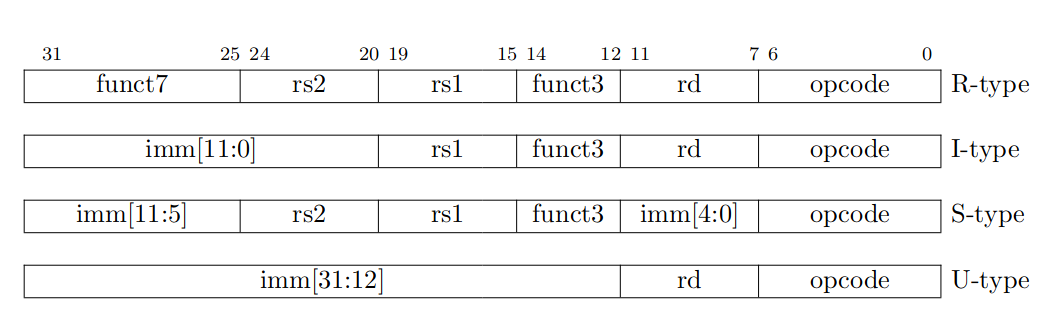
\includegraphics[width=1.0\textwidth]{img/RISCV_4_Commands.png}
    \caption{Основные форматы команд 32-разрядного процессора RISC-V}
    \label{command-01}
\end{figure}
Обозначения на рисунке:
\begin{itemize}
    \item \textbf{opcode} — код операции (6 битов)
    \item \textbf{rs1} --- № регистра-источника (5 битов)
    \item \textbf{rs2} --- № регистра-опреанда (5 битов)
    \item \textbf{rd} --- № регистра-приёмника (5 битов)
    \item \textbf{imm[11:0]} --- непосредственный операнд размером в 12 битов (В случае, когда непосредственное значение определяет «приёмник» (смещен адреса для «близкого» перехода или записи результата в память), 12 битов целиком в поле rd не помещаются, и его приходится «распиливать» (инструкция типа S). Непосредственный операнд всегда знаковый, и его знак всегда приходится на 31-й бит)
    \item \textbf{imm[31:12]} --- непосредственный операнд размером в 20 битов. Используется в инструкциях типа U для заполнения старших двадцати битов регистра (в операциях «далёкого» перехода и как дополнительная инструкция при записи в регистр полного 32-разрядного непосредственного операнда)
    \item \textbf{funct} --- поле функции (6 битов), используется для разных инструкций, у которых код операции одинаковый. Например, все арифметические инструкции типа I имеют одинаковый opcode OP-IMM (чему он равен?), а различаются полем funct. По-видимому, для эффективной реализации R-команд в конвейере удобнее не декодировать опкод, а по-быстрому сравнить его с нулём, и получать значения регистров, параллельно декодируя функцию, чтобы потом её применить.
\end{itemize}

\debate[Примечание]{Ниже представлен альтернативных рисунок из Reference Card с большим числом форматов. На всякий случай. Просто ряд форматов имеют одинаковые поля, но различную семантику. Пока непонятно, что лучше и проще преподносить. Может сказать о второй форме как способ уточнения семантики?}

Щесть базовых типов команд (рисунок~\ref{command-02}):

\begin{figure}[htbp]
    \centering
    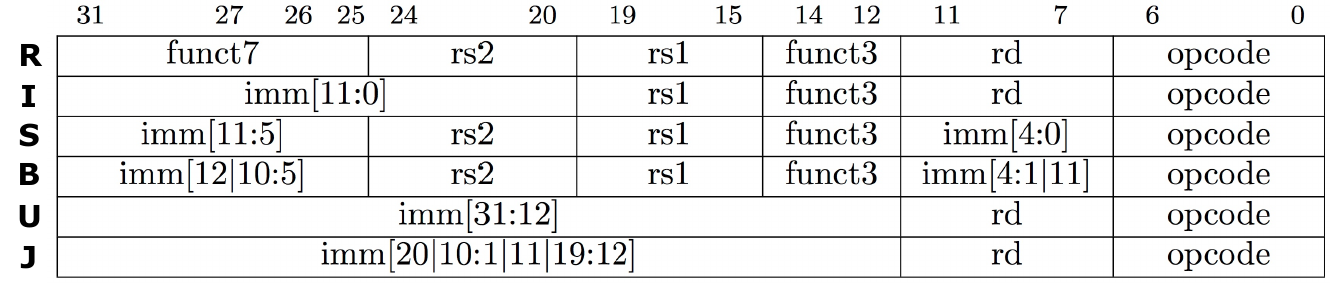
\includegraphics[width=1.0\textwidth]{img/32-bit-instruction-formats.png}
    \caption{Основные форматы команд 32-разрядного процессора RISC-V}
    \label{command-02}
\end{figure}

\section{Базовый набор команд процессора}

Процессор содержит основной набор команд, каждая из который отображается в одну инструкцию на языке ассемблера. Вместе с тем ассемблер, для повышения удобства программирования, дополнительно поддерживает псевдокоманды, каждая из которых может кодировать до нескольких машинных команд или иметь специфические операнды, позволяющие сформировать мнемонику команды, удобную для восприятия человеком.

Арифметические команды представлены в таблице~\ref{table-base-arithmetic}

\begin{table}[h]
    \caption{Арифметические команды набора RV32I}
    \centering
    \begin{tabularx}{\textwidth}{|l|c|X|}
        \hline
        \textbf{Команда} & \textbf{Формат} & \textbf{Описание} \\
        %\hline  \multicolumn{3}{|c|}{\textbf{\textit{Арифметические}}} \\
        \hline \verb|add rd,rs1,rs2| & R & Целочисленное сложение: \verb|rd  = rs1 + rs2| \\
        \hline \verb|addi rd,rs1,int12| & I & Сложение непосредственно с числом: \verb|rd = rs1 + int12| \\
        \hline \verb|sub t1,t2,t3| & R & Subtraction: set t1 to (t2 minus t3) \\
        \hline \verb|lui t1,100000| & U & Load upper immediate: set t1 to 20-bit followed by 12 0s \\
        \hline \verb|auipc rd,100000| & U & Сложение старших 20 разрядов непосредственного числа с \verb|pc|: \verb|rd = pc + int[31:12]| (pc плюс 20-бит непосредственного операнда как старшие разряды 32-разрядного числа, расширенного нулями) \\
        \hline
    \end{tabularx}
    \label{table-base-arithmetic}
\end{table}

Логические команды представлены в таблице~\ref{table-base-logical}

\begin{table}[h]
    \caption{Логические команды набора RV32I}
    \centering
    \begin{tabularx}{\textwidth}{|l|c|X|}
        \hline
        \textbf{Команда} & \textbf{Формат} & \textbf{Описание} \\
        %\hline  \multicolumn{3}{|c|}{\textbf{\textit{Арифметические}}} \\
        \hline \verb|add rd,rs1,rs2| & R & Целочисленное сложение: \verb|rd  = rs1 + rs2| \\
        \hline \verb|addi rd,rs1,int12| & I & Сложение непосредственно с числом: \verb|rd = rs1 + int12| \\
        \hline \verb|sub t1,t2,t3| & R & Subtraction: set t1 to (t2 minus t3) \\
        \hline \verb|lui t1,100000| & U & Load upper immediate: set t1 to 20-bit followed by 12 0s \\
        \hline
    \end{tabularx}
    \label{table-base-logical}
\end{table}


Команды сдвига представлены в таблице~\ref{table-base-shift}

\begin{table}[h]
    \caption{Команды сдвига набора RV32I}
    \centering
    \begin{tabularx}{\textwidth}{|l|c|X|}
        \hline
        \textbf{Команда} & \textbf{Формат} & \textbf{Описание} \\
        \hline \verb|xor t1,t2,t3| & R & Bitwise XOR : Set t1 to bitwise XOR of t2 and t3 \\
        \hline \verb|xori t1,t2,-100| & I & Bitwise XOR immediate : Set t1 to bitwise XOR of t2 and sign-extended   12-bit immediate \\
        \hline \verb|or t1,t2,t3| & R & Bitwise OR : Set t1 to bitwise OR of t2 and t3 \\
        \hline \verb|ori t1,t2,-100| & I & Bitwise OR immediate : Set t1 to bitwise OR of t2 and sign-extended 12-bit immediate \\
        \hline \verb|and rd,rs1,rs2| & R & Поразрядное И: \verb|rd = rs1 & rs2| \\
        \hline \verb|andi rd,rs1,int12| & I & Поразрядное И непосредственно с числом: \verb|rd = rs2 & int12| (с расширением знакового разряда у int12) \\
        \hline
    \end{tabularx}
    \label{table-base-shift}
\end{table}

Команды сравнения представлены в таблице~\ref{table-base-compare}

\begin{table}[h]
    \caption{Команды сравнения набора RV32I}
    \centering
    \begin{tabularx}{\textwidth}{|l|c|X|}
        \hline
        \textbf{Команда} & \textbf{Формат} & \textbf{Описание} \\
        \hline \verb|slt t1,t2,t3| & R & Set less than : If t2 is less than t3, then set t1 to 1 else set t1 to 0 \\
        \hline \verb|slti t1,t2,-100| & I & Set less than immediate : If t2 is less than sign-extended 12-bit immediate, then set t1 to 1 else set t1 to 0 \\
        \hline \verb|sltu t1,t2,t3| & R & Set less than : If t2 is less than t3 using unsigned comparision, then set t1 to 1 else set t1 to 0 \\
        \hline \verb|sltiu t1,t2,-100| & I & Set less than immediate unsigned : If t2 is less than sign-extended 16-bit immediate using unsigned comparison, then set t1 to 1 else set t1 to 0 \\
        \hline
    \end{tabularx}
    \label{table-base-compare}
\end{table}

Команды ветвления представлены в таблице~\ref{table-base-branch}

\begin{table}[h]
    \caption{Команды ветвления набора RV32I}
    \centering
    \begin{tabularx}{\textwidth}{|l|c|X|}
        \hline
        \textbf{Команда} & \textbf{Формат} & \textbf{Описание} \\
        \hline \verb|beq t1,t2,label| & B & Переход, если равно: Переход к оператору по label, если \verb|t1 == t2|. \\
        \hline \verb|bge t1,t2,label| & B & Перейти, если больше или равно: перейти к оператору по label, если \verb|t1 >= t2| \\
        \hline \verb|bgeu t1,t2,label| & B & Переход, если больше или равно для беззнаковых чисел: переход к оператору по адресу метки, если \verb|t1 >= t2| (с беззнаковой интерпретацией)  \\
        \hline \verb|blt t1,t2,label| & B & Переход, если меньше: Переход к оператору по label, если \verb|t1 < t2| \\
        \hline \verb|bltu t1,t2,label| & B & Переход, если меньше для беззнаковых чисел: переход к оператору по label, если \verb|t1 < t2| (с беззнаковой интерпретацией) \\
        \hline \verb|bne t1,t2,label| & B & Переход, если не равно: Переход к оператору по label, если \verb|t1 != t2|. \\
        \hline
    \end{tabularx}
    \label{table-base-branch}
\end{table}

Команды перехода и связывания представлены в таблице~\ref{table-base-jump}

\begin{table}[h]
    \caption{Команды ветвления набора RV32I}
    \centering
    \begin{tabularx}{\textwidth}{|l|c|X|}
        \hline
        \textbf{Команда} & \textbf{Формат} & \textbf{Описание} \\
        \hline \verb|jal t1, target| & J & Jump and link : Set t1 to Program Counter (return address) then jump to statement at target address \\
        \hline \verb|jalr t1, t2, -100| & I & Jump and link register: Set t1 to Program Counter (return address) then jump to statement at t2 + immediate \\
        \hline
    \end{tabularx}
    \label{table-base-jump}
\end{table}

Команды синхронизации представлены в таблице~\ref{table-base-sync}

\begin{table}[h]
    \caption{Команды синхронизации набора RV32I}
    \centering
    \begin{tabularx}{\textwidth}{|l|c|X|}
        \hline
        \textbf{Команда} & \textbf{Формат} & \textbf{Описание} \\
        \hline \verb|fence 1, 1| & I & Ensure that IO and memory accesses before the fence happen before the following IO and memory accesses as viewed by a different thread \\
        \hline \verb|fence.i| & I & Ensure that stores to instruction memory are visible to instruction fetches \\
        \hline
    \end{tabularx}
    \label{table-base-sync}
\end{table}

Команды взаимодействия с окружением представлены в таблице~\ref{table-base-env}

\begin{table}[h]
    \caption{Команды взаимодействия с окружением набора RV32I}
    \centering
    \begin{tabularx}{\textwidth}{|l|c|X|}
        \hline
        \textbf{Команда} & \textbf{Формат} & \textbf{Описание} \\
        \hline \verb|ebreak| & I & Pause execution \\
        \hline \verb|ecall| & I & Issue a system call: Execute the system call specified by value in a7 \\
        \hline
    \end{tabularx}
    \label{table-base-env}
\end{table}

Команды работы с регистром состояния представлены в таблице~\ref{table-base-env}

\begin{table}[h]
    \caption{Команды работы с регистром состояния набора RV32I}
    \centering
    \begin{tabularx}{\textwidth}{|l|c|X|}
        \hline
        \textbf{Команда} & \textbf{Формат} & \textbf{Описание} \\
        \hline \verb|csrrc t0, fcsr, t1| & I & Atomic Read/Clear CSR: read from the CSR into t0 and clear bits of the CSR according to t1 \\
        \hline \verb|srrci t0, fcsr, 10| & I & Atomic Read/Clear CSR Immediate: read from the CSR into t0 and clear bits of the CSR according to a constant \\
        \hline \verb|csrrs t0, fcsr, t1| & I & Atomic Read/Set CSR: read from the CSR into t0 and logical or t1 into the CSR \\
        \hline \verb|csrrsi t0, fcsr, 10| & I & Atomic Read/Set CSR Immediate: read from the CSR into t0 and logical or a constant into the CSR \\
        \hline \verb|csrrw t0, fcsr, t1| & I & Atomic Read/Write CSR: read from the CSR into t0 and write t1 into the CSR \\
        \hline \verb|csrrwi t0, fcsr, 10| & I & Atomic Read/Write CSR Immediate: read from the CSR into t0 and write a constant into the CSR \\
        \hline
    \end{tabularx}
    \label{table-base-env}
\end{table}

Команды загрузки данных представлены в таблице~\ref{table-base-load}

\begin{table}[h]
    \caption{Команды загрузки данных набора RV32I}
    \centering
    \begin{tabularx}{\textwidth}{|l|c|X|}
        \hline
        \textbf{Команда} & \textbf{Формат} & \textbf{Описание} \\
        \hline \verb|lb t1, -100(t2)| & I & Set t1 to sign-extended 8-bit value from effective memory byte address \\
        \hline \verb|lbu t1, -100(t2)| & I & Set t1 to zero-extended 8-bit value from effective memory byte address \\
        \hline \verb|lh t1, -100(t2)| & I & Set t1 to sign-extended 16-bit value from effective memory halfword address \\
        \hline \verb|lhu t1, -100(t2)| & I & Set t1 to zero-extended 16-bit value from effective memory halfword address \\
        \hline \verb|lw t1, -100(t2)| & I & Set t1 to contents of effective memory word address \\
        \hline
    \end{tabularx}
    \label{table-base-load}
\end{table}

Команды выгрузки данных представлены в таблице~\ref{table-base-store}

\begin{table}[h]
    \caption{Команды выгрузки данных набора RV32I}
    \centering
    \begin{tabularx}{\textwidth}{|l|c|X|}
        \hline
        \textbf{Команда} & \textbf{Формат} & \textbf{Описание} \\
        \hline \verb|sb t1, -100(t2)| & S & Store byte : Store the low-order 8 bits of t1 into the effective memory byte address \\
        \hline \verb|sh t1, -100(t2)| & S & Store halfword : Store the low-order 16 bits of t1 into the effective memory halfword address \\
        \hline \verb|sw t1, -100(t2)|& S & Store word : Store contents of t1 into effective memory word address \\
        \hline
    \end{tabularx}
    \label{table-base-store}
\end{table}

Команды умножения, деления, выделения остатка, расширяющие базовый набор, и используемые в эмулятора RARS, представлены в таблице~\ref{table-base-mul}

\begin{table}[h]
    \caption{Команды умножения, деления, вычисления остатка набора RV32I}
    \centering
    \begin{tabularx}{\textwidth}{|l|c|X|}
        \hline
        \textbf{Команда} & \textbf{Формат} & \textbf{Описание} \\
        \hline \verb|mul t1,t2,t3| & R & Multiplication: set t1 to the lower 32 bits of t2*t3 \\
        \hline \verb|mulh t1,t2,t3| & R & Multiplication: set t1 to the upper 32 bits of t2*t3 using signed multiplication \\
        \hline \verb|mulhsu t1,t2,t3| & R & Multiplication: set t1 to the upper 32 bits of t2*t3 where t2 is signed and t3 is unsigned \\
        \hline \verb|mulhu t1,t2,t3| & R & Multiplication: set t1 to the upper 32 bits of t2*t3 using unsigned multiplication \\
        \hline \verb|div t1,t2,t3| & R & Division: set t1 to the result of t2/t3 \\
        \hline \verb|divu t1,t2,t3| & R & Division: set t1 to the result of t2/t3 using unsigned division \\
        \hline \verb|rem t1,t2,t3| & R & Remainder: set t1 to the remainder of t2/t3 \\
        \hline \verb|remu t1,t2,t3| & R & Remainder: set t1 to the remainder of t2/t3 using unsigned division \\
        \hline
    \end{tabularx}
    \label{table-base-mul}
\end{table}

Команды для работы по прерываниям представлены в таблице~\ref{table-base-mul}

\begin{table}[h]
    \caption{Команды для работы с прерываниями эмулятора RARS}
    \centering
    \begin{tabularx}{\textwidth}{|l|c|X|}
        \hline
        \textbf{Команда} & \textbf{Формат} & \textbf{Описание} \\
        \hline
        \hline \verb|uret| & ? & Return from handling an interrupt or exception (to uepc) \\
        \hline \verb|wfi| & ? & Wait for Interrupt \\
        \hline
    \end{tabularx}
    \label{table-base-instructions5}
\end{table}

Введенные обозначения:

int12 --- 12-разрядное целое со знаком

% --- Сопроцессор с плавающей точкой ---
\chapter{Сопроцессор с плавающей точкой}

\section{Система команд сопроцессора}

\debate[Примечание]{Думаю, что имеет смысл, как и в случае базовых команд, разбить на несколько таблиц, сгруппировав по назначению.}

\begin{table}[h]
    \caption{Базовые команды процессора RISC-V (продолжение 1)}
    \centering
    \begin{tabularx}{\textwidth}{|l|X|}
        \hline
        \textbf{Опция} & \textbf{Описание} \\
        \hline \hline
        \hline \verb|fadd.d f1, f2, f3, dyn| & Floating ADD (64 bit): assigns f1 to f2 + f3 \\
        \hline \verb|fadd.s f1, f2, f3, dyn| & Floating ADD: assigns f1 to f2 + f3 \\
        \hline \verb|fclass.d t1, f1| & Classify a floating point number (64 bit) \\
        \hline \verb|fclass.s t1, f1| & Classify a floating point number \\
        \hline \verb|fcvt.d.s f1, f2, dyn| & Convert a float to a double: Assigned the value of f2 to f1 \\
        \hline \verb|fcvt.d.w f1, t1, dyn| & Convert double from integer: Assigns the value of t1 to f1 \\
        \hline \verb|fcvt.d.wu f1, t1, dyn| & Convert double from unsigned integer: Assigns the value of t1 to f1 \\
        \hline \verb|fcvt.s.d f1, f2, dyn| & Convert a double to a float: Assigned the value of f2 to f1 \\
        \hline \verb|fcvt.s.w f1, t1, dyn| & Convert float from integer: Assigns the value of t1 to f1 \\
        \hline \verb|fcvt.s.wu f1, t1, dyn| & Convert float from unsigned integer: Assigns the value of t1 to f1 \\
        \hline \verb|fcvt.w.d t1, f1, dyn| & Convert integer from double: Assigns the value of f1 (rounded) to t1 \\
        \hline \verb|fcvt.w.s t1, f1, dyn| & Convert integer from float: Assigns the value of f1 (rounded) to t1 \\
        \hline \verb|fcvt.wu.d t1, f1, dyn| & Convert unsinged integer from double: Assigns the value of f1 (rounded) to t1 \\
        \hline \verb|fcvt.wu.s t1, f1, dyn| & Convert unsinged integer from float: Assigns the value of f1 (rounded) to t1 \\
        \hline \verb|fdiv.d f1, f2, f3, dyn| & Floating DIVide (64 bit): assigns f1 to f2 / f3 \\
        \hline \verb|fdiv.s f1, f2, f3, dyn| & Floating DIVide: assigns f1 to f2 / f3 \\
        \hline \verb|feq.d t1, f1, f2| & Floating EQuals (64 bit): if f1 = f2, set t1 to 1, else set t1 to 0 \\
        \hline \verb|feq.s t1, f1, f2| & Floating EQuals: if f1 = f2, set t1 to 1, else set t1 to 0 \\
        \hline \verb|fld f1, -100(t1)| & Load a double from memory \\
        \hline \verb|fle.d t1, f1, f2| & Floating Less than or Equals (64 bit): if f1 <= f2, set t1 to 1, else set t1 to 0 \\
        \hline \verb|fle.s t1, f1, f2| & Floating Less than or Equals: if f1 <= f2, set t1 to 1, else set t1 to 0 \\
        \hline
    \end{tabularx}
    \label{table-base-instructions2}
\end{table}

\begin{table}[h]
    \caption{Базовые команды процессора RISC-V (продолжение 2)}
    \centering
    \begin{tabularx}{\textwidth}{|l|X|}
        \hline
        \textbf{Опция} & \textbf{Описание} \\
        \hline \hline
        \hline \verb|flt.d t1, f1, f2| & Floating Less Than (64 bit): if f1 < f2, set t1 to 1, else set t1 to 0 \\
        \hline \verb|flt.s t1, f1, f2| & Floating Less Than: if f1 < f2, set t1 to 1, else set t1 to 0 \\
        \hline \verb|flw f1, -100(t1)| & Load a float from memory \\
        \hline \verb|fmadd.d f1, f2, f3, f4, dynFused| & Multiply Add (64 bit): Assigns f2*f3+f4 to f1 \\
        \hline \verb|fmadd.s f1, f2, f3, f4, dynFused| & Multiply Add: Assigns f2*f3+f4 to f1 \\
        \hline \verb|fmax.d f1, f2, f3| & Floating MAXimum (64 bit): assigns f1 to the larger of f1 and f3 \\
        \hline \verb|fmax.s f1, f2, f3| & Floating MAXimum: assigns f1 to the larger of f1 and f3 \\
        \hline \verb|fmin.d f1, f2, f3| & Floating MINimum (64 bit): assigns f1 to the smaller of f1 and f3 \\
        \hline \verb|fmin.s f1, f2, f3| & Floating MINimum: assigns f1 to the smaller of f1 and f3 \\
        \hline \verb|fmsub.d f1, f2, f3, f4, dynFused| & Multiply Subatract: Assigns f2*f3-f4 to f1 \\
        \hline \verb|fmsub.s f1, f2, f3, f4, dynFused| & Multiply Subatract: Assigns f2*f3-f4 to f1 \\
        \hline \verb|fmul.d f1, f2, f3, dyn| & Floating MULtiply (64 bit): assigns f1 to f2 * f3 \\
        \hline \verb|fmul.s f1, f2, f3, dyn| & Floating MULtiply: assigns f1 to f2 * f3 \\
        \hline \verb|fmv.s.x f1, t1| & Move float: move bits representing a float from an integer register \\
        \hline \verb|fmv.x.s t1, f1| & Move float: move bits representing a float to an integer register \\
        \hline \verb|fnmadd.d f1, f2, f3, f4, dynFused| & Negate Multiply Add (64 bit): Assigns -(f2*f3+f4) to f1 \\
        \hline \verb|fnmadd.s f1, f2, f3, f4, dynFused| & Negate Multiply Add: Assigns -(f2*f3+f4) to f1 \\
        \hline \verb|fnmsub.d f1, f2, f3, f4, dynFused| & Negated Multiply Subatract: Assigns -(f2*f3-f4) to f1 \\
        \hline \verb|fnmsub.s f1, f2, f3, f4, dynFused| & Negated Multiply Subatract: Assigns -(f2*f3-f4) to f1 \\
        \hline \verb|fsd f1, -100(t1)| & Store a double to memory \\
        \hline \verb|fsgnj.d f1, f2, f3| & Floating point sign injection (64 bit): replace the sign bit of f2 with the sign bit of f3 and assign it to f1 \\
        \hline \verb|fsgnj.s f1, f2, f3| & Floating point sign injection: replace the sign bit of f2 with the sign bit of f3 and assign it to f1 \\
        \hline
    \end{tabularx}
    \label{table-base-instructions3}
\end{table}

\begin{table}[h]
    \caption{Базовые команды процессора RISC-V (продолжение 3)}
    \centering
    \begin{tabularx}{\textwidth}{|l|X|}
        \hline
        \textbf{Опция} & \textbf{Описание} \\
        \hline \hline
        \hline \verb|fsgnjn.d f1, f2, f3| & Floating point sign injection (inverted 64 bit): replace the sign bit of f2 with the opposite of sign bit of f3 and assign it to f1 \\
        \hline \verb|fsgnjn.s f1, f2, f3| & Floating point sign injection (inverted): replace the sign bit of f2 with the opposite of sign bit of f3 and assign it to f1 \\
        \hline \verb|fsgnjx.d f1, f2, f3| & Floating point sign injection ( 64 bit): xor the sign bit of f2 with the sign bit of f3 and assign it to f1 \\
        \hline \verb|fsgnjx.s f1, f2, f3| & Floating point sign injection (xor): xor the sign bit of f2 with the sign bit of f3 and assign it to f1 \\
        \hline \verb|fsqrt.d f1, f2, dyn| & Floating SQuare RooT (64 bit): Assigns f1 to the square root of f2 \\
        \hline \verb|fsqrt.s f1, f2, dyn| & Floating SQuare RooT: Assigns f1 to the square root of f2 \\
        \hline \verb|fsub.d f1, f2, f3, dyn| & Floating SUBtract (64 bit): assigns f1 to f2 - f3 \\
        \hline \verb|fsub.s f1, f2, f3, dyn| & Floating SUBtract: assigns f1 to f2 - f3 \\
        \hline \verb|fsw f1, -100(t1)| & Store a float to memory \\
        \hline
    \end{tabularx}
    \label{table-base-instructions4}
\end{table}

% --- Заключене -------------------------------------------
\chapter*{Заключение}
\addcontentsline{toc}{chapter}{Заключение}

%\centering
\framebox[0.8\textwidth][l]{\textit{Продолжение следует...}}

% --- Библиография -------------------------------------------
\begin{thebibliography}{00}
%\addcontentsline{toc}{section}{Литература}

\bibitem
{risc-v}
RISC-V International. Описание архитектуры и ее обоснование.
--- \url{https://riscv.org/}

\bibitem
{Harris}
Сара Л. Харрис, Дэвид Харрис.
Цифровая схемотехника и архитектура компьютера: RISC-V / пер. с англ. В. С. Яценкова, А. Ю. Романова; под ред. А. Ю. Романова. --- М.: ДМК Пресс, 2021. --- 810 с.

\bibitem
{Borin}
Edson Borin
An Introduction to Assembly Programming with RISC-V /
Document version: May 9, 2022
--- \url{https://riscv-programming.org/}


\bibitem
{kur-2022}
Курячий Георгий. Архитектура и язык ассемблера RISC-V. Весна 2022.
--- \url{http://uneex.ru/LecturesCMC/ArchitectureAssembler2022}

\bibitem
{aps-git}
Семестровый забег "Архитектур процессорных систем"
--- \url{https://github.com/MPSU/APS}

\bibitem
{kur-youtube-2022}
[UNИX] Архитектура и язык ассемблера RISC-V. Видео лекции. Весна 2022.
--- \url{https://www.youtube.com/playlist?list=PL6kSdcHYB3x6cjkby4H1RuRMzfbEGSNBi}

\bibitem
{aps-youtube}
Архитектуры процессорных систем
--- \url{https://www.youtube.com/c/%D0%90%D0%9F%D0%A1%D0%9F%D0%BE%D0%BF%D0%BE%D0%B2}

\bibitem
{RARS}
RARS -- RISC-V Assembler and Runtime Simulator
--- \url{https://github.com/TheThirdOne/rars}

\bibitem
{Ripes}
Ripes. A visual computer architecture simulator and assembly code editor.
--- \url{https://github.com/mortbopet/Ripes}

\bibitem
{QtRvSim}
QtRvSim–RISC-V CPU simulator for education
--- \url{https://github.com/cvut/qtrvsim}

\bibitem
{Goossens}
Goossens Bernard.
Guide to Computer Processor Architecture. A RISC-V Approach, with High-Level Synthesis.
--- Springer Nature. Switzerland AG --- 2023.

\bibitem
{Booch92}
Буч Г.
Объектно-ориентированное проектирование с примерами применения. /Пер. с англ.
--- М.: Конкорд, 1992. --- 519 с.

\bibitem
{Gay}
Gay Warren.
RISC-V Assembly Language Programming. Using ESP32-C3 and QEMU.
--- Elektor International Media B.V. --- 2022.

\bibitem
{Booch98}
Буч Г.
Объектно-ориентированный анализ и проектирование с примерами приложений на C++, 2-е изд./Пер. с англ.
--- М.: «Издательства Бином», СПб: «Невский диалект», 1998 г. --- 560 с., ил.

\bibitem
{ERD-dict}
Англо-русско-немецко-французский толковый словарь по вычислительной технике и обработке данных, 4132 термина.
Под. ред. А.А. Дородницына. М.: 1978. --- 416 с.

\bibitem
{Gagarina}
Гагарина Л.Г., Кононова А.И.
Архитектура вычислительных систем и Ассемблер с приложением методических указаний к лабораторным работам. Учебное пособие.
--- М.: СОЛОН-Пресс, 2019. --- 368 с.

\bibitem
{elf64}
Формат файла ELF64.
--- \url{https://uclibc.org/docs/elf-64-gen.pdf}

\bibitem
{Plantz}
Plantz Robert G.
Introduction to Computer Organization.
--- 2022

\bibitem
{gdb-stollman}
Ричард Столмен, Роланд Пеш, Стан Шебс и др.
Отладка с помощью GDB.
--- 2000

\bibitem
{gdb-zeller}
Андреас Целлер
Почему не работают программы.
--- М.: Эксмо, 2011. --- 560 с.

\bibitem
{gdb-dive-into-systems}
Suzanne J. Matthews, Tia Newhall, Kevin C. Webb.
Dive into Systems.
--- 2022

\bibitem
{round-up}
Округление. Статья в Википедии.
--- \url{https://ru.wikipedia.org/wiki/%D0%9E%D0%BA%D1%80%D1%83%D0%B3%D0%BB%D0%B5%D0%BD%D0%B8%D0%B5}

\bibitem
{c-lang}
Прохоренок Н.А.
Язык С. Самое необходимое.
--- СПб.: БХВ-Петербург, 2020. --- 480 с.

\bibitem
{nasm-x64}
Йо Ван Гуй.
Программирование на ассемблере x64: от начального уровня до профессионального использования AVX.
--- М.: ДМК Пресс, 2021. --- 332 с.

\bibitem
{wsl}
Установка Linux на Windows с помощью WSL
--- \url{https://docs.microsoft.com/ru-ru/windows/wsl/install}

\bibitem
{vir-box}
Установка Linux на Virtualbox.
--- \url{https://losst.ru/ustanovka-linux-na-virtualbox}

\bibitem
{System-V}
System V Application Binary Interface AMD64 Architecture Processor Supplement (With LP64 and ILP32 Programming Models). Version 1.0. --- 2018.
--- \url{https://github.com/hjl-tools/x86-psABI/wiki/x86-64-psABI-1.0.pdf}



\end{thebibliography}


\end {document}
